%%%%%%%%%%%%%%%%%%%%%%%%%%%%%%%%%%%%%%%%%%%%%%%%%%%%%%%%%%%%%%%%%%%%%%%%%%
%                                                                        %
%                            INTRODUCTION                                %
%                                                                        %
%%%%%%%%%%%%%%%%%%%%%%%%%%%%%%%%%%%%%%%%%%%%%%%%%%%%%%%%%%%%%%%%%%%%%%%%%%
\subsection{Methods}
\begin{frame}{Energy Deposition and Simulations with GEANT4}
GEANT4 is a free toolkit for the simulation of particles as they travel through matter\cite{agostinelli_geant4simulation_2003}
\label{G4Main}
  \begin{columns}[onlytextwidth]
  \begin{column}{0.49\textwidth}
    \centering
    \begin{figure}
    \includegraphics[width=\textwidth]{GEANT4AnnotatedGeo_EnergyDepEvent}
    \end{figure}
  \end{column}
  \begin{column}{0.49\textwidth}
    \centering
    \begin{figure}
	  \includegraphics[width=\textwidth]{GEANT4AnnotatedGeo_GS20SimGeo}
    \end{figure}
  \end{column}
  \end{columns}
\hyperlink{G4Intro}{\beamerbutton{Energy Deposition with GEANT4}}
\end{frame}
%%%%%%%%%%%%%%%%%%%%%%%%%%%%%%%%%%%%%%%%%%%%%%%%%%%%%%%%%%%%%%%%%%%%%%%%%%
\begin{frame}{Single Collision Energy Loss Spectra}
  \begin{figure}
    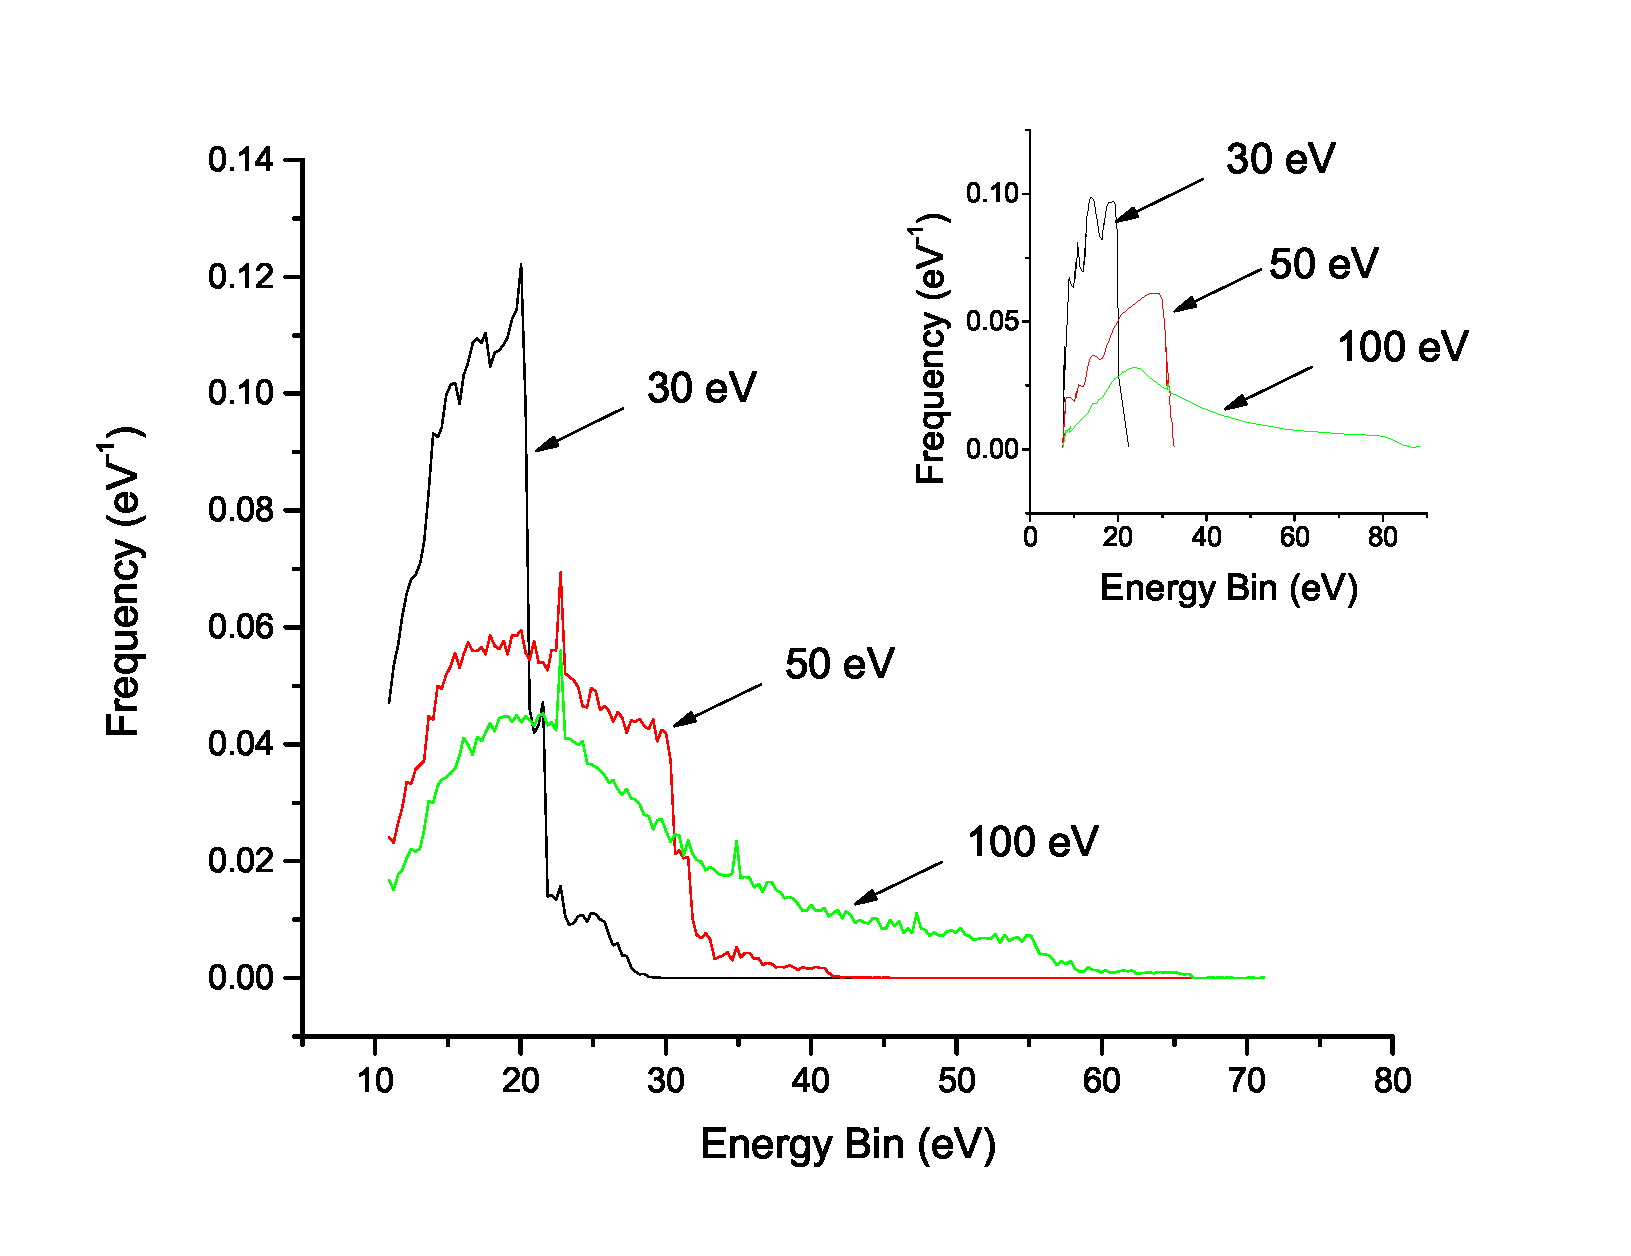
\includegraphics[width=\textwidth]{SingleCollsionEnergyLoss_Turner}
    \caption{Single Collision Energy Loss in Water\cite{turner_comparative_1982}}
  \end{figure}
\vspace{2mm}
Discrepancies are in the resolution of cross section data
\end{frame}
%%%%%%%%%%%%%%%%%%%%%%%%%%%%%%%%%%%%%%%%%%%%%%%%%%%%%%%%%%%%%%%%%%%%%%%%%%
\begin{frame}{Energy Deposition in Polymers}
  \begin{columns}[onlytextwidth]
  \begin{column}{0.5\textwidth}
    \centering
    \begin{figure}
    	\includegraphics[width=\textwidth]{G4EDep_LightYield_Neutron}
    \end{figure}
      Neutron
  \end{column}
  \begin{column}{0.5\textwidth}
    \centering
    \begin{figure}
    	\includegraphics[width=\textwidth]{G4EDep_LightYield_Co60}
    \end{figure}
      \iso[60]{Co} Gamma
  \end{column}
  \end{columns}
\end{frame}
%%%%%%%%%%%%%%%%%%%%%%%%%%%%%%%%%%%%%%%%%%%%%%%%%%%%%%%%%%%%%%%%%%%%%%%%%%
%                                                                        %
%                               RESULTS                                  %
%                                                                        %
%%%%%%%%%%%%%%%%%%%%%%%%%%%%%%%%%%%%%%%%%%%%%%%%%%%%%%%%%%%%%%%%%%%%%%%%%%
\subsection{Results}
%%%%%%%%%%%%%%%%%%%%%%%%%%%%%%%%%%%%%%%%%%%%%%%%%%%%%%%%%%%%%%%%%%%%%%%%%%
\begin{frame}{Electron Range and Energy Distributions}
  Very differnet interactions between the alpha, triton, and gammas
  \begin{figure}
    \centering
    \includegraphics[height=0.75\textheight,keepaspectratio]{ElectronRangeAndEnergyDist}
  \end{figure}
\end{frame}
%%%%%%%%%%%%%%%%%%%%%%%%%%%%%%%%%%%%%%%%%%%%%%%%%%%%%%%%%%%%%%%%%%%%%%%%%%
\begin{frame}
  \label{EDepScint}
  \begin{figure}
    \centering
    \includegraphics[height=0.7\textheight]{LightSim_AlphaTritonElectron}
  \end{figure}
  GEANT4 simulated light output of alpha, tritons and electrons in polystyrene
  \hyperlink{ScintEnergyDep}{\beamerbutton{Scintillation and Energy Deposition}}
\end{frame}
%%%%%%%%%%%%%%%%%%%%%%%%%%%%%%%%%%%%%%%%%%%%%%%%%%%%%%%%%%%%%%%%%%%%%%%%%%
\begin{frame}{Simulated Optical Photon Yield of GS20}
  \begin{figure}
    \centering
    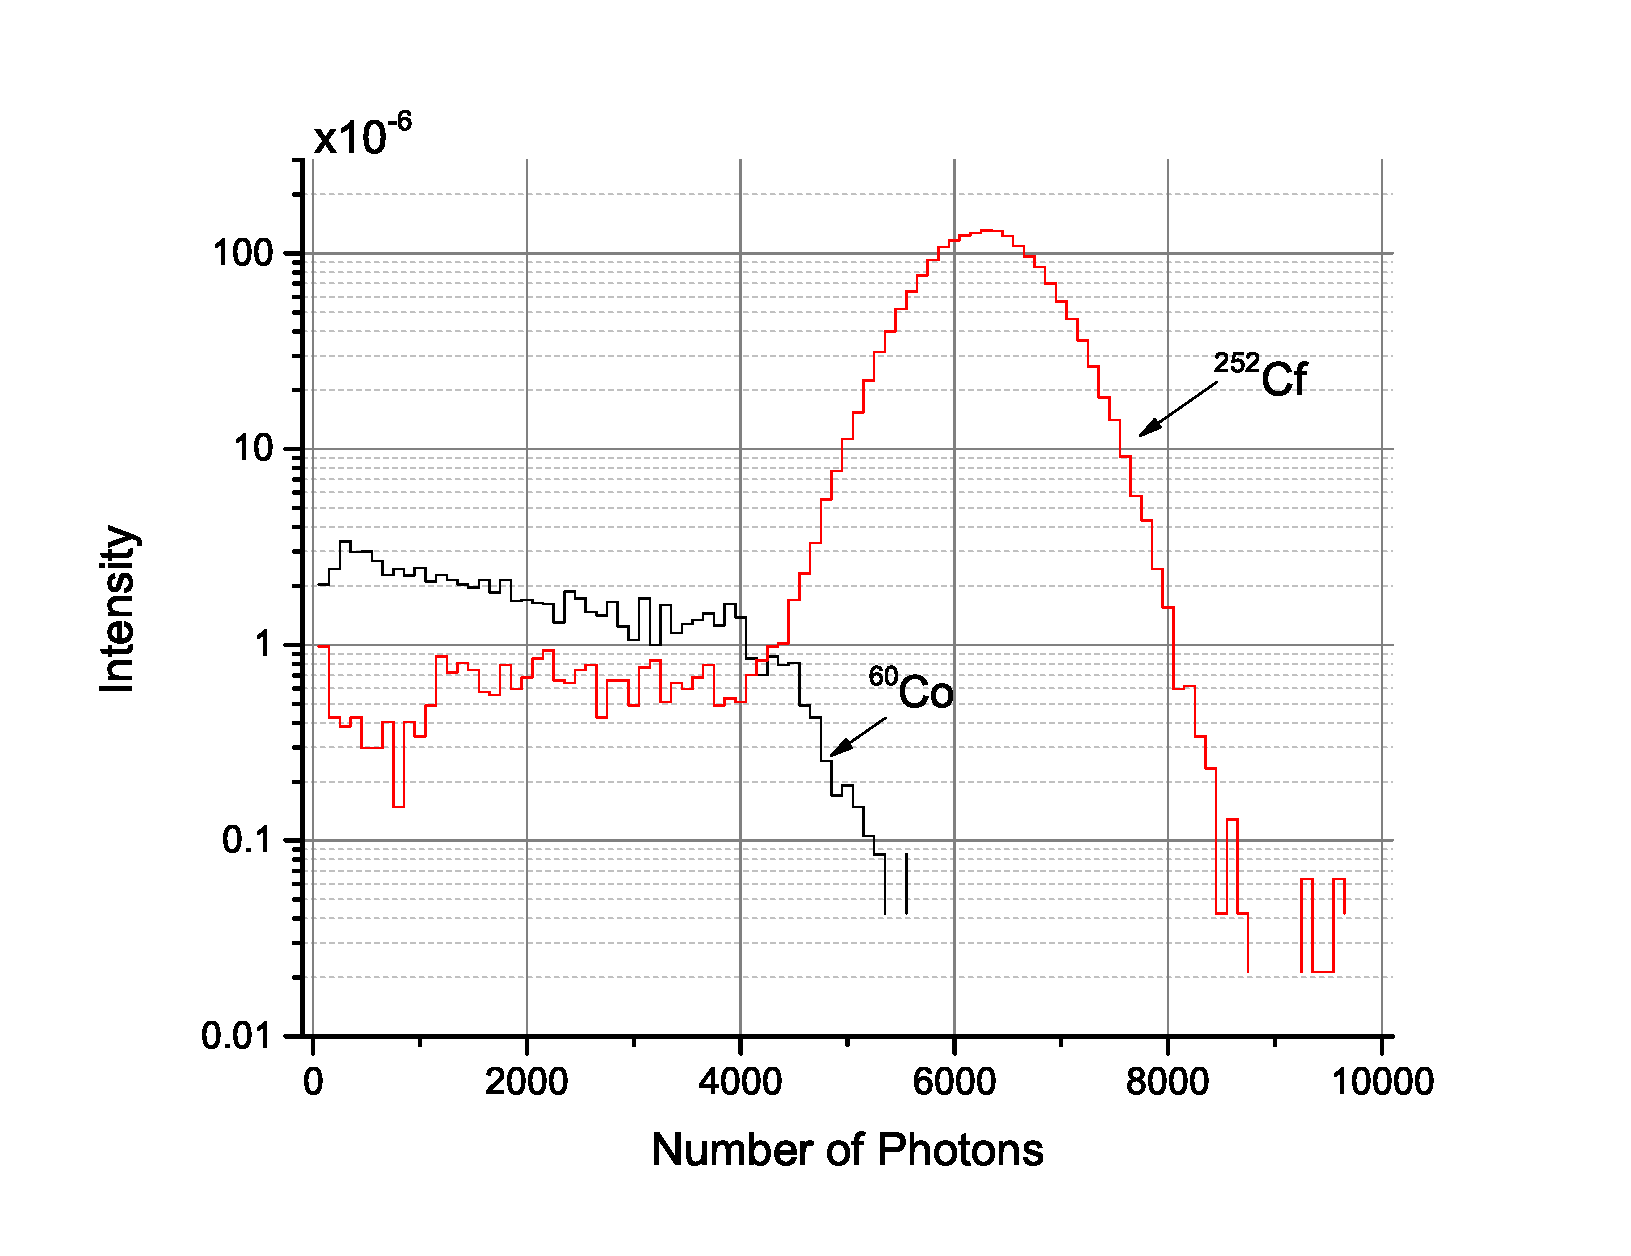
\includegraphics[width=\textwidth]{LightValidation_GS20}
  \end{figure}
\end{frame}
%%%%%%%%%%%%%%%%%%%%%%%%%%%%%%%%%%%%%%%%%%%%%%%%%%%%%%%%%%%%%%%%%%%%%%%%%%
\begin{frame}{Simulated Optical Photon Yield of Polystyrene}
  \begin{figure}
    \centering
    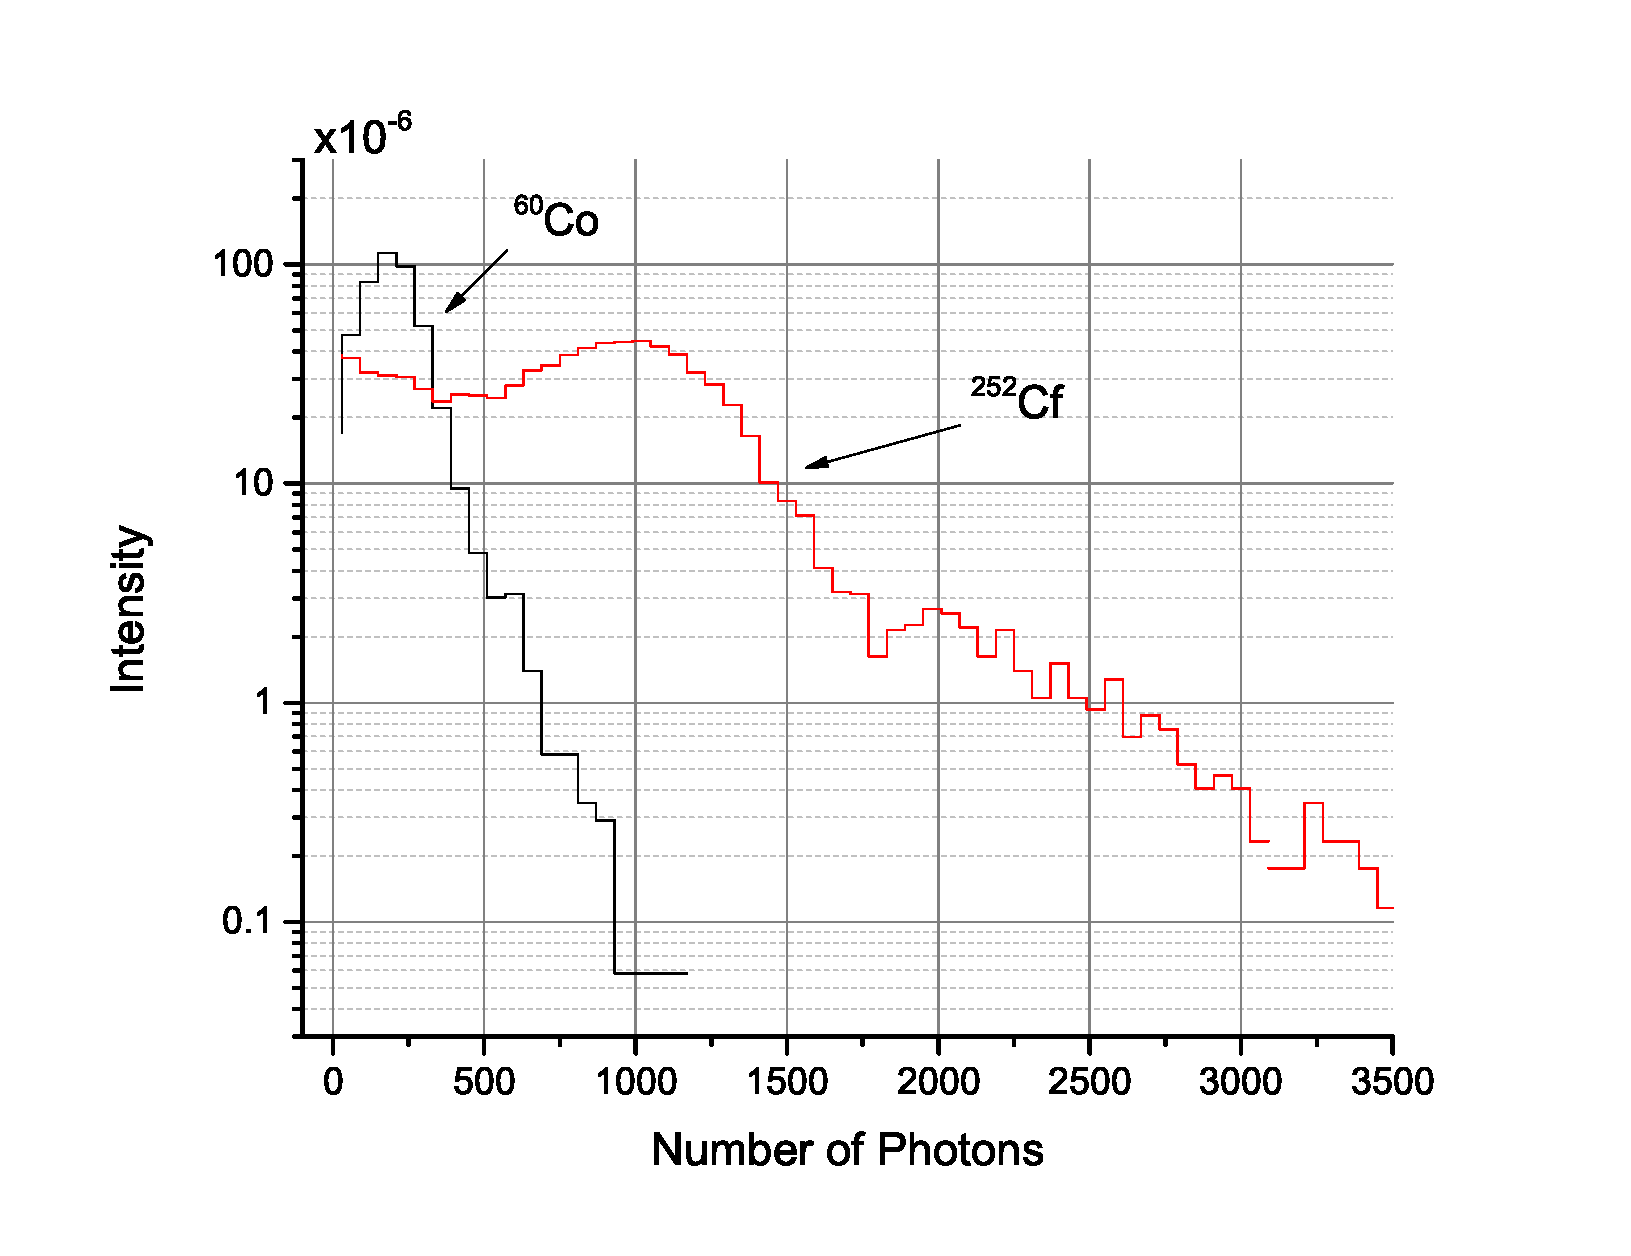
\includegraphics[width=\textwidth]{LightValidation_PS}
  \end{figure}
  \vspace{2.5cm}
\end{frame}
%%%%%%%%%%%%%%%%%%%%%%%%%%%%%%%%%%%%%%%%%%%%%%%%%%%%%%%%%%%%%%%%%%%%%%%%%%
